\documentclass[10pt,a4paper]{article}
\usepackage[margin=2.2cm]{geometry}
\usepackage{graphicx,booktabs,amsmath,multirow}
\usepackage[table]{xcolor}
\usepackage{caption}
\usepackage[hidelinks]{hyperref}
\usepackage{microtype}
\captionsetup{font=small,labelfont=bf,skip=4pt}
\setlength{\tabcolsep}{4pt}
\newcommand{\ci}[2]{{\footnotesize[#1,\,#2]}}

\title{Execution-Grounded Audit of a Pre-Built Code Graph and Node Embeddings for Repository-Level Agentic Coding}
\author{Saurav Bellam\\ \small The University of Texas at Austin \quad \texttt{sauravbellam@utexas.edu}}
\date{Draft, 11 October 2026}

\begin{document}
\maketitle

\begin{abstract}
Agentic-coding benchmarks increasingly ship a pre-computed code graph and node embeddings so that an agent can navigate a repository through tools rather than raw text. We audit one such release---127 commit-level graphs and 256-d node vectors covering 129 tasks drawn from \textsc{fastapi}, \textsc{rich}, \textsc{requests} and \textsc{httpx}---against the source code itself and against the real call graph recorded by executing each task's tests under a tracer. Every one of the 45{,}492 \texttt{async def} definitions is missing from the graph (0\%), although 81 of 711 gold-patch symbols are asynchronous. The provided \texttt{calls} relation holds 37.9\% of the executed non-test call edges \ci{34.4}{42.5} (\textsc{fastapi} 75.5\%, \textsc{rich} 26.2\%) and only 21.4\% of its edges whose endpoints ran were actually observed; 83\% of the unobserved edges have no reference to the callee in the caller's source. The harness's bare-name resolver returns a different, same-named node for 41\% of present functions and 65\% of absent asynchronous ones. The node vectors are a text embedding of an unidentified encoder (best public candidate: cosine 0.07): identical text yields identical vectors across commits (99.6\% at cosine $\ge$0.99), and a graph neural network gains nothing from structure beyond text in 124 of 127 graphs. Consequently, plain BM25 over the repository source surfaces the gold file in the top five for 65.9\% of tasks against 33.3\% for the harness's retrieval ($p<10^{-5}$, McNemar). Where the gold function is a node, the executed path from the failing tests reaches it in 95.8\% of tasks, so a corrected typed graph with dynamic edges is a sound substitute.
\end{abstract}

\section{Introduction}
Repository-level coding agents are routinely given a \emph{map}: a graph whose nodes are modules, classes and functions and whose edges are calls, plus an embedding per node for similarity search. The competition archive studied here provides exactly this, consumed through three tools of the \texttt{swegemma}~0.2.7 harness: \texttt{resolve\_node\_name} (four tiers: exact, suffix, case-insensitive, substring), \texttt{get\_neighbor} (edge type filtered by equality) and \texttt{search\_similar\_code} (cosine over the provided vectors). A map that omits definitions, invents edges or embeds the wrong thing silently caps what any agent built on it can do. We ask four questions with executable evidence: (i) is every definition a node, and what do the tools return when it is not? (ii) does the static \texttt{calls} relation match the real call graph? (iii) what produced the vectors and what does cosine track? (iv) does any of this matter for finding the fix location from the issue text?

The archive contains 127 non-empty graphs (422\,MB), 127 embedding files (468\,MB), 130 snapshots (21.5\,GB) and 129 tasks (\textsc{fastapi} 67, \textsc{rich} 48, \textsc{requests} 13, \textsc{httpx} 1). Experiments ran on Debian~13 with Python~3.13.5 (the harness's version); task-level rates carry Wilson intervals, pooled ratios task-cluster bootstrap intervals, and paired comparisons use the exact McNemar test.

\section{Method}
\paragraph{A1, static census.} Every \texttt{.py} file of each snapshot is parsed with \texttt{ast}; each definition (sync function, async function, class, nested def) is checked for a node of the same id, in source and test files separately. For each definition the harness's resolver is replayed on the bare and qualified name, recording whether it returns the definition itself, a wrong node (and which tier produced it, and whether it is a test), or nothing. Per task we map gold-patch hunks to functions, extract identifiers from the issue text, and compute the graph distance $d$ from issue-mentioned nodes to gold nodes and the lexical visibility $v$ (BM25 rank of the gold file over the snapshot source).

\paragraph{A2, execution oracle.} For each task: unpack the snapshot, build a fresh virtual environment with an editable install, apply the test patch, run pytest \emph{pre-fix} under a \texttt{sys.setprofile}/\texttt{threading.setprofile} tracer, apply the gold patch and run again. The tracer records every repository function executed per test and every caller$\to$callee edge, direct or through library frames. A task is \emph{usable} when both runs are clean and at least one expected fail-to-pass test is confirmed. Static edges are compared with the pre-fix trace: \emph{representable recall} (dynamic edges between existing nodes that the graph holds), \emph{agent-facing recall} (also counting edges to absent definitions), \emph{observed precision} (static edges whose endpoints both ran and that were seen), and the cause of every miss.

\paragraph{A3/A3b, embeddings.} Vector statistics; re-embedding of 200 sampled nodes in 10 graphs with EmbeddingGemma-300m, EmbeddingGemma-2 and all-MiniLM-L6-v2 (text, name, id, name+text; with and without documented prompts; identification threshold mean cosine $\ge$0.99); a text-identity check across the 3{,}358 same-repository graph pairs; and a GNN sweep on all 127 graphs (two-layer mean aggregation, 300 epochs, 80/20 node split) with \emph{structural}, \emph{text} (hashed bag of tokens) and \emph{both} feature sets under two objectives: \emph{fit} (predict the provided vector of held-out nodes) and \emph{linkpred} (learn from edges only, align by orthogonal Procrustes, score held-out $k$-NN overlap).

\paragraph{A4/A5, similarity and retrieval.} AUROC of cosine for call-adjacent, containment, same-module, name-overlap and gold co-change pairs against random pairs; composition of each node's ten nearest neighbours. Retrieval of the gold node (Hit@10) and gold file (Hit@5) from the issue text under five modes: resolved identifier anchors only (a0); the harness (anchors plus cosine ranking, a); harness plus one-hop call neighbours (d); BM25 over graph node text (b); BM25 over the real snapshot source (e).

\paragraph{A6--A8.} A corrected typed graph per commit (\texttt{contains}, \texttt{imports}, \texttt{inherits}, \texttt{calls\_static}, \texttt{calls\_dynamic}, \texttt{tests}); an id reconciliation of provided nodes against source definitions; and an audit classifying every captured, missed and unconfirmed edge by how the callee appears in the caller's source.

\section{Results}

\subsection{Coverage of the provided graphs}
The 127 graphs hold 367{,}985 nodes and 452{,}588 edges of a single type, \texttt{calls}. Figure~\ref{fig:census} shows presence by definition kind. Sync functions in source files are complete (90{,}792/90{,}792); classes 97.8\%; nested definitions 78.4\% (stored flattened). \textbf{Asynchronous functions are absent without exception}: 0 of 45{,}492 across all files, 0 of 28{,}113 in source files (Wilson upper bound 0.01\%), 0 of 45{,}399 in \textsc{fastapi}, 0 of 93 in \textsc{httpx}; 10{,}995 async definitions sit in modules that have no node at all. Id reconciliation explains the remaining non-async gaps: 1{,}425 \textsc{requests} functions (19.8\% of its sync functions) and 1{,}279 \textsc{fastapi} classes exist under a \emph{class-dropped} id (\texttt{module.method} rather than \texttt{module.Class.method}), and \textsc{requests} graphs carry 268 nodes matching no definition.

\begin{figure}[t]\centering
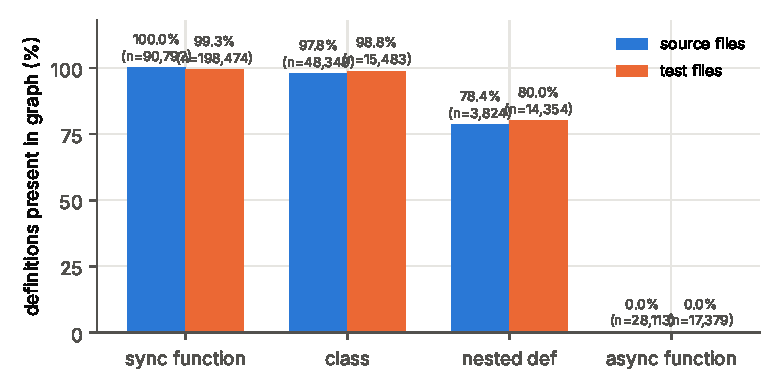
\includegraphics[width=0.72\linewidth]{figs/fig1_census.pdf}
\caption{Definitions present as graph nodes, by kind and file type (127 graphs).}
\label{fig:census}
\end{figure}

The graphs are also structurally sparse where it matters (Figure~\ref{fig:structure}). Half of all nodes (186{,}994; 50.8\%) have no edge; in \textsc{fastapi} 68.7\% of nodes per graph are isolated and 68.4\% are test-file nodes. Between 8.5\% (\textsc{fastapi}) and 29.8\% (\textsc{httpx}) of \texttt{calls} edges are containment pseudo-edges (target id prefixed by source id), not calls; \textsc{fastapi} graphs average 35 self-loops.

\begin{figure}[t]\centering
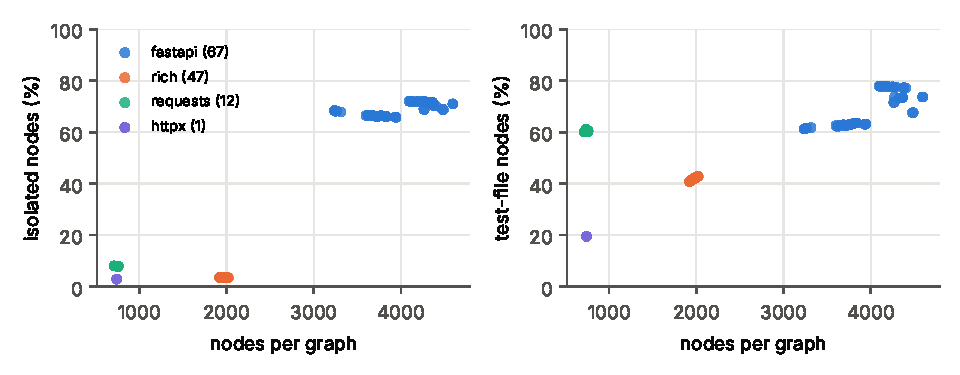
\includegraphics[width=0.8\linewidth]{figs/fig2_graph_structure.pdf}
\caption{Per-graph share of isolated nodes (left) and test-file nodes (right) against graph size.}
\label{fig:structure}
\end{figure}

\paragraph{Gold symbols.} Of 711 gold-patch symbols, 470 (66.1\%, \ci{62.6}{69.5}) are nodes; 184 are new symbols introduced by the patch and cannot be in a base-commit graph; 81 are asynchronous and \textbf{one} is present (1.2\%). Twenty-two tasks (17.1\%) fix an async function---31.3\% of \textsc{fastapi} tasks (21/67) and the \textsc{httpx} task. Eleven tasks have no gold node in the graph at all.

\subsection{What the resolver returns}
Figure~\ref{fig:resolver} replays the harness's name resolution. A bare-name query for a function that \emph{is} a node returns a different node with the same short name in 41.2\% of 287{,}841 cases (\textsc{fastapi} 46.6\%, \textsc{httpx} 62.0\%, \textsc{rich} 28.5\%, \textsc{requests} 17.6\%), and 73{,}723 of those wrong answers are test functions; for classes the rate is 47.9\%. For an absent async function the bare name resolves to a wrong node in 65.4\% of 56{,}487 queries (28{,}961 by suffix, 6{,}413 by substring, 1{,}550 case-insensitive; 26{,}851 of the targets are test nodes) and to nothing in 34.6\%. Qualified names avoid this (5.3\% wrong for present functions, 97.2\% ``no match'' for absent async ones), but issue text rarely contains them: of 1{,}014 identifiers extracted from the 129 issues, 578 resolve to nothing, 219 by suffix, 195 by substring, 17 case-insensitively and 5 exactly; 121 land on test nodes. At task level, a harness-style query for the gold function returns a wrong node in 21 tasks (16.3\%; \textsc{fastapi} 28.4\%).

\begin{figure}[t]\centering
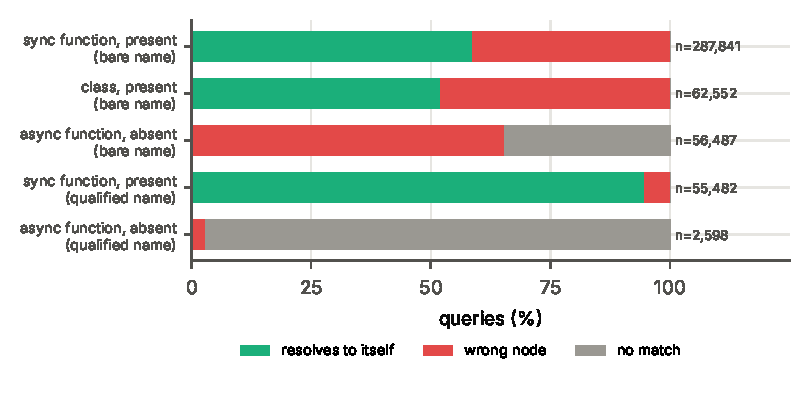
\includegraphics[width=0.7\linewidth]{figs/fig9_resolver.pdf}
\caption{Replaying the four-tier resolver on every definition (127 graphs).}
\label{fig:resolver}
\end{figure}

\subsection{The static \texttt{calls} relation against execution}
All 129 test and gold patches applied exactly. Run classes: 114 clean, 9 collection errors, 4 \textsc{requests} tasks with no collectable tests, 2 import errors. Four \textsc{rich} tasks were killed on the first attempt (10--17 minutes, up to 36\,GB) and recovered with a 60\,s per-test timeout, \texttt{rich\_4006} only after deselecting four hung tests. Of 488 expected fail-to-pass tests, 189 were confirmed, 174 already passed pre-fix and 118 could not be collected pre-fix; 55 tasks had every expected test confirmed. \textbf{91 tasks (70.5\%, \ci{62.2}{77.7}) are usable} (\textsc{fastapi} 45, \textsc{rich} 39, \textsc{requests} 7).

\begin{table}[t]\centering\small
\caption{Recall of executed call edges and observed precision of static edges, usable tasks, pre-fix traces, direct calls. Intervals: task-cluster bootstrap.}
\label{tab:recall}
\begin{tabular}{llrrr}
\toprule
scope & population & representable recall & agent-facing recall & observed precision\\
\midrule
non-test & all 91 tasks & 37.9\% \ci{34.4}{42.5} (5{,}430/14{,}331) & 35.3\% & 21.4\% \ci{20.0}{22.8}\\
non-test & \textsc{fastapi} (45) & 75.5\% \ci{74.2}{77.1} & -- & 16.5\%\\
non-test & \textsc{rich} (39) & 26.2\% \ci{25.6}{26.9} & -- & 23.1\%\\
non-test & \textsc{requests} (7) & 43.3\% \ci{42.5}{45.4} & -- & 34.3\%\\
gold-incident & all 91 tasks & 57.8\% \ci{40.7}{70.0} (603/1{,}043) & 50.4\% & --\\
non-test & strict 55 tasks & 35.9\% & 33.7\% & 21.3\%\\
non-test & all 125 analysed & 39.7\% & 36.6\% & 21.6\%\\
\bottomrule
\end{tabular}
\end{table}

Table~\ref{tab:recall} and Figure~\ref{fig:recall} give the oracle comparison. The graph holds 37.9\% of the real non-test call edges (per-task mean 53.5\%, \ci{49.4}{58.2}; the pooled figure is dominated by \textsc{rich}'s dense traces). Of the misses, 89.3\% are between nodes that both exist; absent nested definitions account for 7.0\% and absent async functions for 3.6\% overall but 28.4\% in \textsc{fastapi}. Edges incident to a gold function fare better (57.8\%) but with wide uncertainty. Precision is low: of 37{,}433 static edges whose endpoints both executed, 8{,}013 (21.4\%) were observed. The target tests execute 16.7\% of non-test nodes.

\begin{figure}[t]\centering
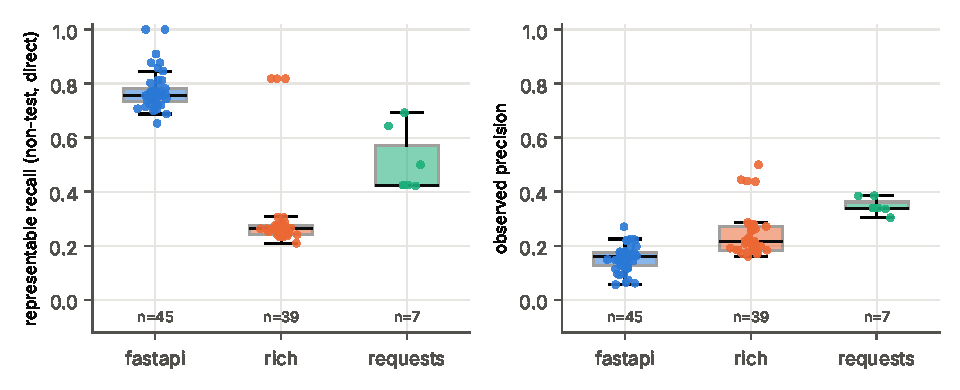
\includegraphics[width=0.78\linewidth]{figs/fig3_recall_precision.pdf}
\caption{Per-task representable recall (left) and observed precision (right) of the provided \texttt{calls} relation, usable tasks.}
\label{fig:recall}
\end{figure}

\paragraph{Why edges are missed or spurious.} Figure~\ref{fig:audit} classifies the 7{,}640 captured, 12{,}231 missed and 35{,}017 unconfirmed non-test edges by how the callee appears in the caller's source. Captured edges are overwhelmingly explicit bare-name calls or instantiations (88.6\% have an explicit call site). Missed edges are method calls through \texttt{self}/\texttt{cls} (15.9\%) or another object (23.4\%), names passed without a call (callbacks, decorators; 28.3\%) and implicit dunders such as \texttt{\_\_init\_\_} or \texttt{\_\_rich\_console\_\_} (17.3\%); the generator emits none of the first kind at all. Among unconfirmed edges, \textbf{56.1\% have no reference to the callee anywhere in the caller and 26.7\% mention it only inside a string or comment}, so 82.8\% are spurious by construction (\textsc{requests} 96\%, \textsc{fastapi} 88\%, \textsc{rich} 76\%); only 11.0\% have an explicit call site that the tests simply did not exercise.

\begin{figure}[t]\centering
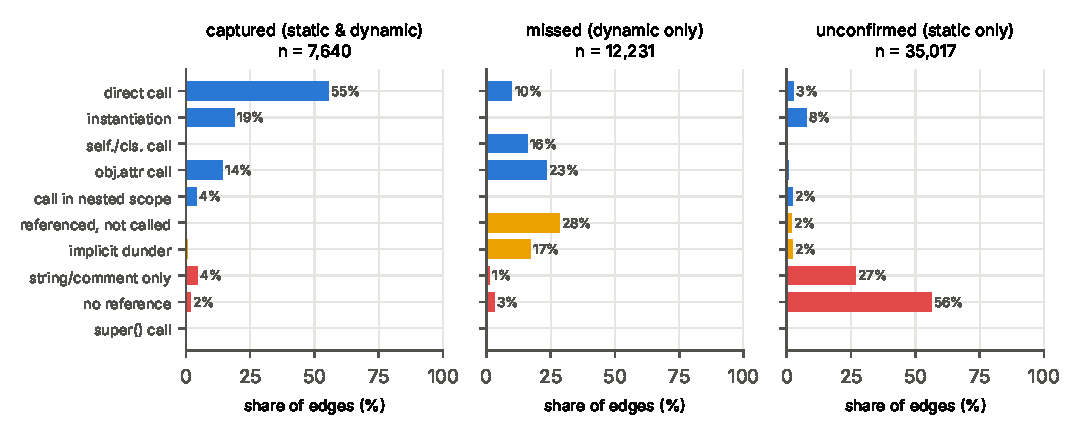
\includegraphics[width=\linewidth]{figs/fig4_edge_audit.pdf}
\caption{How the callee appears in the caller's source, by edge population (non-test, distinct edges). Red: no code reference.}
\label{fig:audit}
\end{figure}

\paragraph{Reachability.} In 72 of the 91 usable tasks (79.1\%, \ci{69.7}{86.2}) the gold function is a node and is executed by a fail-to-pass test; in 3 it is executed but absent. From the executed entry functions, the gold function is reachable along directed static edges in 69 of 72 tasks (95.8\%) and is itself an entry in 32 (Figure~\ref{fig:reach}); from a test \emph{node} of the graph it is reachable in only 5 tasks, because tests added by the test patch are never base-graph nodes.

\begin{figure}[t]\centering
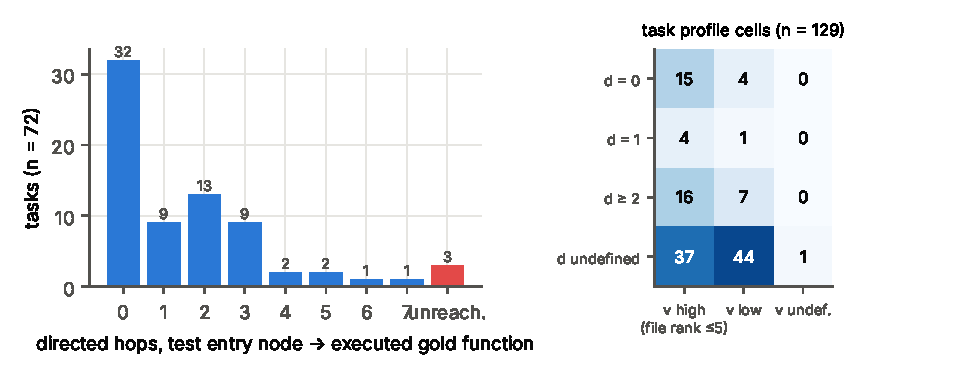
\includegraphics[width=0.8\linewidth]{figs/fig8_reach_cells.pdf}
\caption{Left: directed hops from executed entry function to executed gold function (72 tasks). Right: tasks by graph distance $d$ and lexical visibility $v$ (129 tasks).}
\label{fig:reach}
\end{figure}

\subsection{The node vectors}
The vectors are 256-d, one per node, not unit-norm (mean norm 4.5--5.4) and strongly anisotropic: mean cosine to the mean vector 0.87 (\textsc{fastapi}) to 0.95 (\textsc{rich}), first principal component 44--75\% of variance, mean pairwise cosine 0.75--0.91. No candidate encoder reproduces them: best mean cosine 0.073 (EmbeddingGemma-300m, name variant, document prompt), 0.015 (EmbeddingGemma-2), 0.036 (all-MiniLM-L6-v2); no vector reached 0.95; pairwise Spearman $\le$0.12. Free-text embedding retrieval could therefore not be evaluated.

Three tests settle what the vectors encode. (1) Across 3{,}358 same-repository graph pairs, nodes with byte-identical text have cosine $\ge$0.99 in 99.55\% of cases (worst pair 98.4\%), 5th percentile 0.9996; a pre-registered exact-equality rule (90.0\% at cosine exactly 1) fired on float32 noise and was replaced. Same text with changed neighbours gives 0.971 (unchanged: 0.9998), a small context effect. (2) In the \emph{fit} objective (Figure~\ref{fig:gnn}, left) text alone closes the most of the gap above the mean-vector baseline in every repository (\textsc{rich} 0.88, \textsc{fastapi} 0.67, \textsc{requests} 0.74, \textsc{httpx} 0.92); adding structure lowers held-out cosine by 0.002--0.037 and helps in only 3 of 127 graphs, by at most 0.0013. (3) In \emph{linkpred} (right), embeddings trained only on the graph's edges recover none of the vectors' neighbourhoods ($k$-NN@10 overlap 0.005--0.016, at the random-control level) while text recovers 0.20--0.44. The vectors are thus a text embedding of an unidentified encoder, with the context effect most economically attributed to a text window wider than the node body. A further 16.7\% of nodes per graph (31\% in \textsc{fastapi}) carry an exact duplicate vector.

\begin{figure}[t]\centering
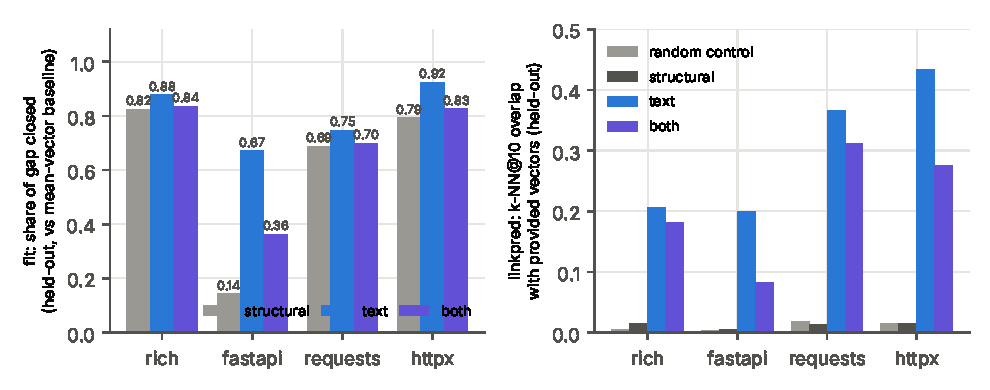
\includegraphics[width=0.9\linewidth]{figs/fig6_gnn.pdf}
\caption{GNN sweep, 127 graphs. Left: held-out gap closed when predicting provided vectors. Right: $k$-NN@10 overlap of edge-only embeddings with the provided vectors.}
\label{fig:gnn}
\end{figure}

\paragraph{What cosine tracks.} Call-adjacent pairs are separable from random pairs (AUROC 0.898, mean cosine 0.988 vs 0.830), as are containment pairs (0.903) and gold co-change pairs (0.806, 51 graphs); same-module (0.682) and name-overlap pairs (0.675) less so (Figure~\ref{fig:sim}). The practical picture is different: of a node's ten nearest neighbours, 45--67\% are test-file nodes in \textsc{fastapi}, \textsc{rich} and \textsc{requests}, 30--49\% share its module and at most 3\% are call neighbours. \texttt{search\_similar\_code} returns code that reads alike, usually a test.

\begin{figure}[t]\centering
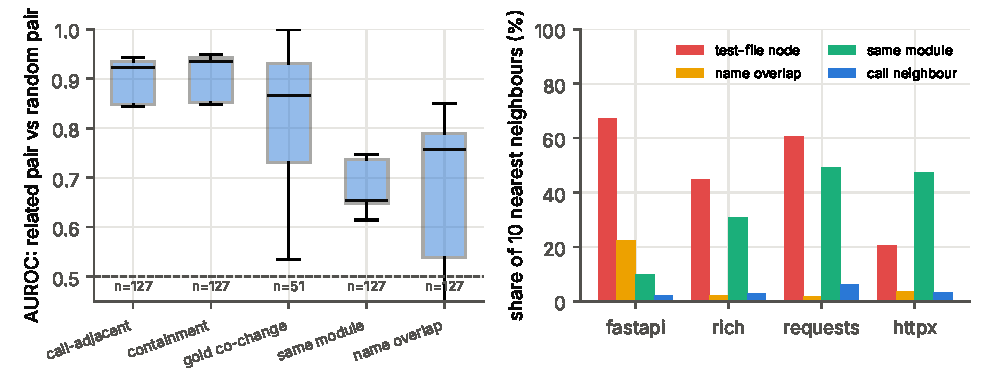
\includegraphics[width=0.9\linewidth]{figs/fig7_similarity.pdf}
\caption{Left: AUROC of cosine for related vs random pairs. Right: composition of the ten nearest neighbours.}
\label{fig:sim}
\end{figure}

\subsection{Retrieval of the fix location}
Figure~\ref{fig:retrieval} and Table~\ref{tab:retrieval} compare retrieval modes over all 129 tasks (a miss when no gold node exists). The harness mode places the gold node in the top ten for 24.0\% of tasks and the gold file in the top five for 33.3\%, and returns \emph{nothing} for 54 tasks (41.9\%) whose issue text yields no resolvable anchor; cosine ranking on top of the anchors adds one node and three files, and one-hop call expansion two files. BM25 over graph node text raises file Hit@5 to 48.8\% ($p=0.0017$). BM25 over the real source, which also sees the omitted async functions, reaches 41.1\% node Hit@10 and 65.9\% file Hit@5 (harness vs source BM25: node $p=5.9\times10^{-5}$, 4 vs 26 discordant tasks; file $p<10^{-5}$, 5 vs 47). The ordering holds in each repository: file Hit@5 \textsc{fastapi} 17$\to$39 of 67, \textsc{rich} 16$\to$33 of 48, \textsc{requests} 9$\to$12 of 13.

\begin{table}[t]\centering\small
\caption{Retrieval of the gold node and file from the issue text, 129 tasks (Wilson 95\% intervals).}
\label{tab:retrieval}
\begin{tabular}{lrrrr}
\toprule
mode & gold node Hit@10 & gold file Hit@5 & MRR & empty\\
\midrule
a0 anchors only & 23.3\% \ci{16.8}{31.3} & 31.0\% \ci{23.7}{39.4} & 0.170 & 54\\
a harness (anchors + cosine) & 24.0\% \ci{17.5}{32.1} & 33.3\% \ci{25.8}{41.9} & 0.174 & 54\\
d harness + 1-hop calls & 24.0\% \ci{17.5}{32.1} & 34.9\% \ci{27.2}{43.4} & 0.175 & 54\\
b BM25, graph node text & 29.5\% \ci{22.3}{37.8} & 48.8\% \ci{40.4}{57.4} & 0.170 & 0\\
e BM25, snapshot source & \textbf{41.1\%} \ci{33.0}{49.7} & \textbf{65.9\%} \ci{57.4}{73.5} & \textbf{0.232} & 0\\
\bottomrule
\end{tabular}
\end{table}

\begin{figure}[t]\centering
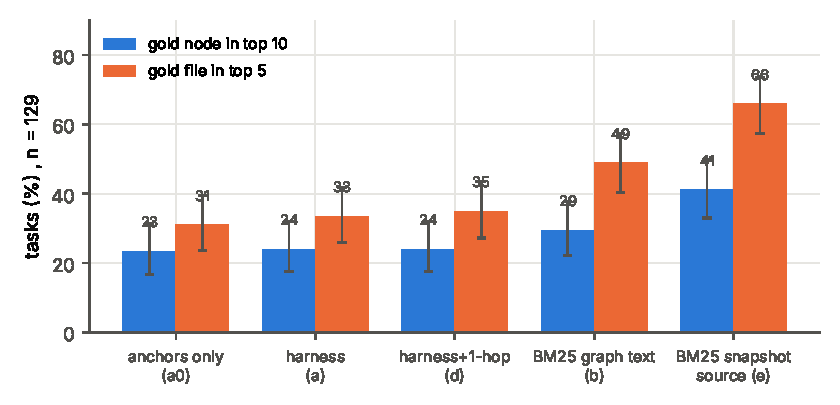
\includegraphics[width=0.72\linewidth]{figs/fig5_retrieval.pdf}
\caption{Retrieval modes over all 129 tasks with Wilson intervals.}
\label{fig:retrieval}
\end{figure}

\subsection{A corrected graph}
Rebuilding each commit from source yields graphs with typed edges and the missing kinds: per \textsc{fastapi} graph 6{,}146 nodes (1{,}008 async functions, 1{,}163 modules, 827 classes), 4{,}989 \texttt{contains}, 2{,}605 \texttt{imports}, 408 \texttt{inherits}, 2{,}214 \texttt{calls\_static}, 422 \texttt{calls\_dynamic} (from the traces) and 567 \texttt{tests} edges, with 2{,}199 nodes the provided graph lacks; \textsc{rich} 2{,}208 nodes and 979 dynamic edges, \textsc{requests} 890 and 801, \textsc{httpx} 885 and 494. Only 47 tasks (36.4\%) have a defined $d$ (Figure~\ref{fig:reach}, right); 82 issues mention no resolvable node, while 72 have a lexically visible gold file.

\section{Discussion}
The generator skipped every \texttt{async def}, so for the asynchronous third of \textsc{fastapi} tasks the fix site is not on the map, and the resolver's suffix and substring tiers then route the agent to a same-named test function rather than reporting absence. Where nodes exist, the \texttt{calls} relation appears to come from name matching rather than analysis of call sites: it never records \texttt{self.method()} or dunder dispatch, which make up most of the real edges, and four in five of its unobserved edges point to callees the caller never names. The embeddings add a third, independent limitation: they encode text only, and the dominant text in the corpus is tests, so similarity search mostly returns tests. The practical consequence is the retrieval result: a lexical index over the raw files beats every graph-based mode on every metric, partly because it sees what the graph cannot.

Two results are encouraging. First, the dynamic oracle shows that when the gold function is a node, the real execution path from the failing tests reaches it in 96\% of tasks, usually within two hops, so a correct call graph is a useful instrument. Second, the corrected graph recovers the missing kinds and adds test provenance.

\paragraph{Limitations.} Tests ran in virtual environments with network access rather than the harness's container; subprocesses spawned by tests are not traced; dynamic edges through library frames are excluded from the corrected graph. Thirty-eight tasks are not usable for the execution comparison (20 clean runs with no expected fail-to-pass test, 3 with none confirmed, 9 collection errors, 2 import errors, 4 without collectable tests); \texttt{rich\_4006} needed hung-test deselection. Graphs within a repository are near-identical commits, so per-graph intervals are not independent, and \textsc{httpx} contributes one task. The encoder's input window is inferred, not observed, and the 80-edge hand-review sample of the edge audit has not yet been labelled.

\section*{Reproducibility}
All scripts, per-task raw outputs (traces, junit XML, environment freezes), checksums of the code as run and of \texttt{tasks.jsonl}, and the corrected graphs are in the results archive; each pooled number carries its numerator, denominator and interval in the corresponding summary file.

\begin{thebibliography}{9}
\bibitem{swebench} C. E. Jimenez et al. SWE-bench: Can language models resolve real-world GitHub issues? \emph{ICLR}, 2024.
\bibitem{bm25} S. Robertson and H. Zaragoza. The probabilistic relevance framework: BM25 and beyond. \emph{Found.\ Trends Inf.\ Retr.}, 3(4), 2009.
\bibitem{wilson} E. B. Wilson. Probable inference, the law of succession, and statistical inference. \emph{J.\ Am.\ Stat.\ Assoc.}, 22, 1927.
\bibitem{mcnemar} Q. McNemar. Note on the sampling error of the difference between correlated proportions or percentages. \emph{Psychometrika}, 12, 1947.
\bibitem{graphsage} W. Hamilton, Z. Ying and J. Leskovec. Inductive representation learning on large graphs. \emph{NeurIPS}, 2017.
\bibitem{gemma} Google DeepMind. EmbeddingGemma model card, 2025.
\end{thebibliography}

\end{document}
